\documentclass[a4paper]{oblivoir}
%%%Default packages
\usepackage{amsmath,amssymb,amsthm,kotex,tabu,graphicx,pifont}
\usepackage{../kswrapfig}

\usepackage{gensymb} %\degree

%%%More packages
%\usepackage{caption,subcaption}
%\usepackage[perpage]{footmisc}
%
\usepackage[skipabove=10pt,innertopmargin=10pt,nobreak=true]{mdframed}

\usepackage[inline]{enumitem}
\setlist[enumerate,1]{label=(\arabic*)}
\setlist[enumerate,2]{label=(\alph*)}

\usepackage{multicol}
\setlength{\columnsep}{30pt}
\setlength{\columnseprule}{1pt}
%
%\usepackage{forest}
%\usetikzlibrary{shapes.geometric,arrows.meta,calc}
%
%%%defi theo exam prob rema proo
%이 환경들 아래에 문단을 쓸 경우 살짝 들여쓰기가 되므로 \hspace{-.7em}가 필요할 수 있다.

\newcounter{num}
\newcommand{\defi}[1]
{\noindent\refstepcounter{num}\textbf{정의 \arabic{num})} #1\par\noindent}
\newcommand{\theo}[1]
{\noindent\refstepcounter{num}\textbf{정리 \arabic{num})} #1\par\noindent}
\newcommand{\revi}[1]
{\noindent\refstepcounter{num}\textbf{복습 \arabic{num})} #1\par\noindent}
\newcommand{\exam}[1]
{\bigskip\bigskip\noindent\refstepcounter{num}\textbf{예시 \arabic{num})} #1\par\noindent}
\newcommand{\prob}[1]
{\bigskip\bigskip\noindent\refstepcounter{num}\textbf{문제 \arabic{num})} #1\par\noindent}
\newcommand{\rema}[1]
{\bigskip\bigskip\noindent\refstepcounter{num}\textbf{참고 \arabic{num})} #1\par\noindent}
\newcommand{\proo}
{\bigskip\noindent\textsf{증명)}}

\newenvironment{talign}
 {\let\displaystyle\textstyle\align}
 {\endalign}
\newenvironment{talign*}
 {\let\displaystyle\textstyle\csname align*\endcsname}
 {\endalign}
%
%%%Commands

\newcommand{\procedure}[1]{\begin{mdframed}\vspace{#1\textheight}\end{mdframed}}

\newcommand\an[1]{\par\bigskip\noindent\textbf{문제 \ref{#1})}\par\noindent}

\newcommand\ann[2]{\par\bigskip\noindent\textbf{문제 \ref{#1})}\:\:#2\par\medskip\noindent}

\newcommand\ans[1]{\begin{flushright}\textbf{답 : }#1\end{flushright}}

\newcommand\anssec[1]{\bigskip\bigskip\noindent{\large\bfseries#1}}

\newcommand{\pb}[1]%\Phantom + fBox
{\fbox{\phantom{\ensuremath{#1}}}}

\newcommand\ba{\,|\,}

\newcommand\ovv[1]{\ensuremath{\overline{#1}}}
\newcommand\ov[2]{\ensuremath{\overline{#1#2}}}
%
%%%% Settings
%\let\oldsection\section
%
%\renewcommand\section{\clearpage\oldsection}
%
%\let\emph\textsf
%
%\renewcommand{\arraystretch}{1.5}
%
%%%% Footnotes
%\makeatletter
%\def\@fnsymbol#1{\ensuremath{\ifcase#1\or
%*\or **\or ***\or
%\star\or\star\star\or\star\star\star\or
%\dagger\or\dagger\dagger\or\dagger\dagger\dagger
%\else\@ctrerr\fi}}
%
%\renewcommand{\thefootnote}{\fnsymbol{footnote}}
%\makeatother
%
%\makeatletter
%\AtBeginEnvironment{mdframed}{%
%\def\@fnsymbol#1{\ensuremath{\ifcase#1\or
%*\or **\or ***\or
%\star\or\star\star\or\star\star\star\or
%\dagger\or\dagger\dagger\or\dagger\dagger\dagger
%\else\@ctrerr\fi}}%
%}   
%\renewcommand\thempfootnote{\fnsymbol{mpfootnote}}
%\makeatother
%
%%% 객관식 선지
\newcommand\one{\ding{172}}
\newcommand\two{\ding{173}}
\newcommand\three{\ding{174}}
\newcommand\four{\ding{175}}
\newcommand\five{\ding{176}}
\usepackage{tabto,pifont}
%\TabPositions{0.2\textwidth,0.4\textwidth,0.6\textwidth,0.8\textwidth}

\newcommand\taba[5]{\par\noindent
\one\:{#1}
\tabto{0.2\textwidth}\two\:\:{#2}
\tabto{0.4\textwidth}\three\:\:{#3}
\tabto{0.6\textwidth}\four\:\:{#4}
\tabto{0.8\textwidth}\five\:\:{#5}}

\newcommand\tabb[5]{\par\noindent
\one\:{#1}
\tabto{0.33\textwidth}\two\:\:{#2}
\tabto{0.67\textwidth}\three\:\:{#3}\medskip\par\noindent
\four\:\:{#4}
\tabto{0.33\textwidth}\five\:\:{#5}}

\newcommand\tabc[5]{\par\noindent
\one\:{#1}
\tabto{0.5\textwidth}\two\:\:{#2}\medskip\par\noindent
\three\:\:{#3}
\tabto{0.5\textwidth}\four\:\:{#4}\medskip\par\noindent
\five\:\:{#5}}

\newcommand\tabd[5]{\par\noindent
\one\:{#1}\medskip\par\noindent
\two\:\:{#2}\medskip\par\noindent
\three\:\:{#3}\medskip\par\noindent
\four\:\:{#4}\medskip\par\noindent
\five\:\:{#5}}
%
%%%% fonts
%
%\usepackage{fontspec, xunicode, xltxtra}
%\setmainfont[]{은 바탕}
%\setsansfont[]{은 돋움}
%\setmonofont[]{은 바탕}
%\XeTeXlinebreaklocale "ko"
\begin{document}

\begin{center}
미니테스트 3 관련 문제들
\end{center}
%%
\section{경우의 수}
%
\begin{minipage}{.65\textwidth}
\begin{Exercise}
오른쪽 그림의 2개의 영역을 서로 다른 4가지 색 \(a\), \(b\), \(c\), \(d\)로 칠하려고 한다.
같은 색을 중복해서 사용해도 좋으나 인접한 영역은 서로 다른 색으로 칠할 때, 칠하는 방법의 수를 구하시오.
\end{Exercise}
\end{minipage}
\quad
\begin{minipage}{.25\textwidth}
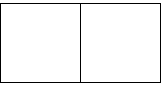
\includegraphics[width=.5\textwidth]{1}
\end{minipage}

\bigskip\noindent
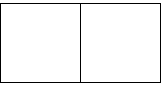
\includegraphics[width=.2\textwidth]{1}\quad
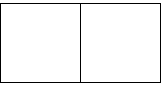
\includegraphics[width=.2\textwidth]{1}\quad
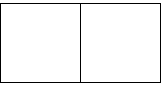
\includegraphics[width=.2\textwidth]{1}\quad
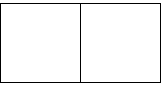
\includegraphics[width=.2\textwidth]{1}\\[5pt]
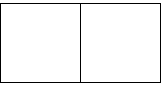
\includegraphics[width=.2\textwidth]{1}\quad
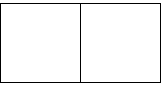
\includegraphics[width=.2\textwidth]{1}\quad
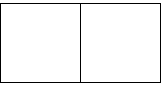
\includegraphics[width=.2\textwidth]{1}\quad
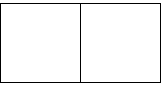
\includegraphics[width=.2\textwidth]{1}\\[5pt]
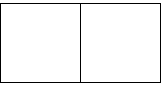
\includegraphics[width=.2\textwidth]{1}\quad
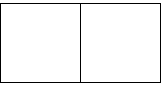
\includegraphics[width=.2\textwidth]{1}\quad
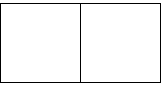
\includegraphics[width=.2\textwidth]{1}\quad
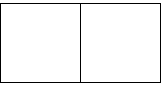
\includegraphics[width=.2\textwidth]{1}\\[5pt]
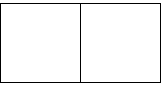
\includegraphics[width=.2\textwidth]{1}\quad
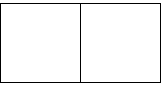
\includegraphics[width=.2\textwidth]{1}\quad
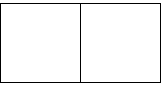
\includegraphics[width=.2\textwidth]{1}\quad
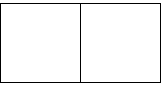
\includegraphics[width=.2\textwidth]{1}

\ans{12}

\noindent
%
\begin{minipage}{.65\textwidth}
\begin{Exercise}
오른쪽 그림의 3개의 영역을 서로 다른 4가지 색 \(a\), \(b\), \(c\), \(d\)로 칠하려고 한다.
같은 색을 중복해서 사용해도 좋으나 인접한 영역은 서로 다른 색으로 칠할 때, 칠하는 방법의 수를 구하시오.
\end{Exercise}
\end{minipage}
\quad
\begin{minipage}{.25\textwidth}
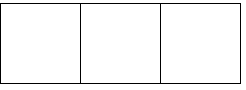
\includegraphics[width=.5\textwidth]{2}
\end{minipage}

\bigskip\noindent
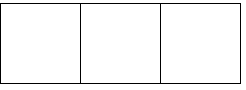
\includegraphics[width=.2\textwidth]{2}\quad
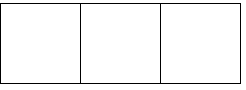
\includegraphics[width=.2\textwidth]{2}\quad
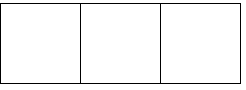
\includegraphics[width=.2\textwidth]{2}\quad
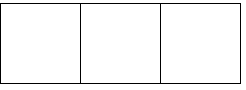
\includegraphics[width=.2\textwidth]{2}\\[5pt]
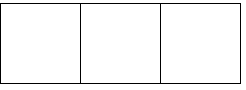
\includegraphics[width=.2\textwidth]{2}\quad
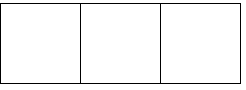
\includegraphics[width=.2\textwidth]{2}\quad
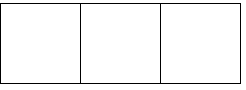
\includegraphics[width=.2\textwidth]{2}\quad
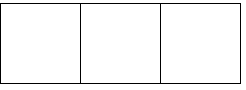
\includegraphics[width=.2\textwidth]{2}\\[5pt]
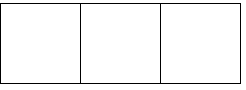
\includegraphics[width=.2\textwidth]{2}\quad
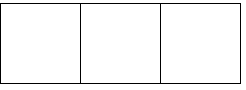
\includegraphics[width=.2\textwidth]{2}\quad
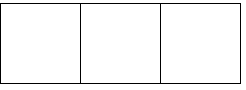
\includegraphics[width=.2\textwidth]{2}\quad
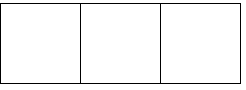
\includegraphics[width=.2\textwidth]{2}\\[5pt]
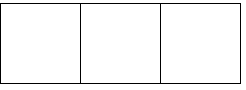
\includegraphics[width=.2\textwidth]{2}\quad
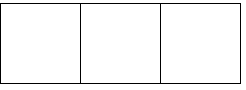
\includegraphics[width=.2\textwidth]{2}\quad
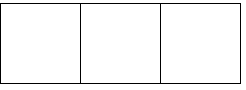
\includegraphics[width=.2\textwidth]{2}\quad
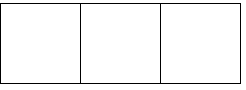
\includegraphics[width=.2\textwidth]{2}\\[5pt]
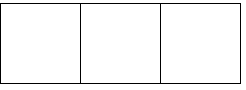
\includegraphics[width=.2\textwidth]{2}\quad
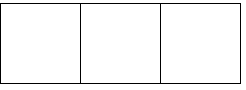
\includegraphics[width=.2\textwidth]{2}\quad
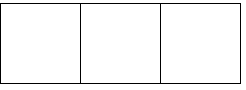
\includegraphics[width=.2\textwidth]{2}\quad
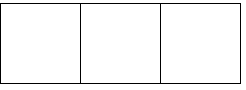
\includegraphics[width=.2\textwidth]{2}\\[5pt]
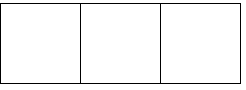
\includegraphics[width=.2\textwidth]{2}\quad
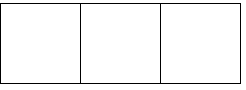
\includegraphics[width=.2\textwidth]{2}\quad
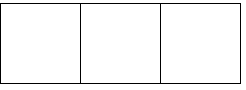
\includegraphics[width=.2\textwidth]{2}\quad
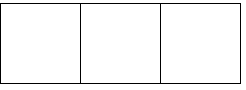
\includegraphics[width=.2\textwidth]{2}\\[5pt]
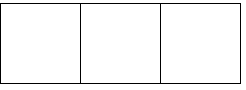
\includegraphics[width=.2\textwidth]{2}\quad
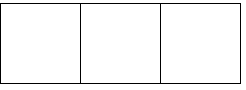
\includegraphics[width=.2\textwidth]{2}\quad
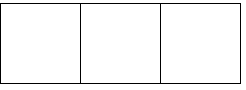
\includegraphics[width=.2\textwidth]{2}\quad
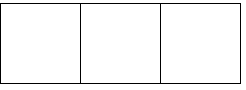
\includegraphics[width=.2\textwidth]{2}\\[5pt]
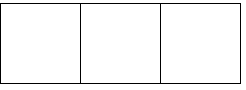
\includegraphics[width=.2\textwidth]{2}\quad
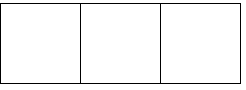
\includegraphics[width=.2\textwidth]{2}\quad
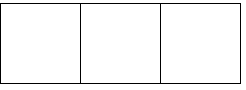
\includegraphics[width=.2\textwidth]{2}\quad
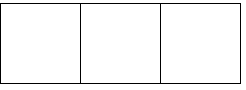
\includegraphics[width=.2\textwidth]{2}\\[5pt]
\includegraphics[width=.2\textwidth]{2}\quad
\includegraphics[width=.2\textwidth]{2}\quad
\includegraphics[width=.2\textwidth]{2}\quad
\includegraphics[width=.2\textwidth]{2}\\[5pt]
\includegraphics[width=.2\textwidth]{2}\quad
\includegraphics[width=.2\textwidth]{2}\quad
\includegraphics[width=.2\textwidth]{2}\quad
\includegraphics[width=.2\textwidth]{2}\\[5pt]
\includegraphics[width=.2\textwidth]{2}\quad
\includegraphics[width=.2\textwidth]{2}\quad
\includegraphics[width=.2\textwidth]{2}\quad
\includegraphics[width=.2\textwidth]{2}\\[5pt]
\includegraphics[width=.2\textwidth]{2}\quad
\includegraphics[width=.2\textwidth]{2}\quad
\includegraphics[width=.2\textwidth]{2}\quad
\includegraphics[width=.2\textwidth]{2}\\[5pt]
\includegraphics[width=.2\textwidth]{2}\quad
\includegraphics[width=.2\textwidth]{2}\quad
\includegraphics[width=.2\textwidth]{2}\quad
\includegraphics[width=.2\textwidth]{2}\\[5pt]

\ans{36}

%
\begin{minipage}{.65\textwidth}
\begin{Exercise}
오른쪽 그림의 4개의 영역을 서로 다른 4가지 색 \(a\), \(b\), \(c\), \(d\)로 칠하려고 한다.
같은 색을 중복해서 사용해도 좋으나 인접한 영역은 서로 다른 색으로 칠할 때, 칠하는 방법의 수를 구하시오.
\end{Exercise}
\end{minipage}
\quad
\begin{minipage}{.25\textwidth}
\includegraphics[width=.5\textwidth]{3}
\end{minipage}

\ans{108}

%
\begin{minipage}{.65\textwidth}
\begin{Exercise}
오른쪽 그림의 3개의 영역을 서로 다른 4가지 색 \(a\), \(b\), \(c\), \(d\)로 칠하려고 한다.
같은 색을 중복해서 사용해도 좋으나 인접한 영역은 서로 다른 색으로 칠할 때, 칠하는 방법의 수를 구하시오.
\end{Exercise}
\end{minipage}
\quad
\begin{minipage}{.25\textwidth}
\includegraphics[width=.5\textwidth]{4}
\end{minipage}

\bigskip\noindent
\includegraphics[width=.1\textwidth]{4}\quad
\includegraphics[width=.1\textwidth]{4}\quad
\includegraphics[width=.1\textwidth]{4}\quad
\includegraphics[width=.1\textwidth]{4}\quad
\includegraphics[width=.1\textwidth]{4}\quad
\includegraphics[width=.1\textwidth]{4}\quad
\includegraphics[width=.1\textwidth]{4}\quad
\includegraphics[width=.1\textwidth]{4}\\[5pt]
\includegraphics[width=.1\textwidth]{4}\quad
\includegraphics[width=.1\textwidth]{4}\quad
\includegraphics[width=.1\textwidth]{4}\quad
\includegraphics[width=.1\textwidth]{4}\quad
\includegraphics[width=.1\textwidth]{4}\quad
\includegraphics[width=.1\textwidth]{4}\quad
\includegraphics[width=.1\textwidth]{4}\quad
\includegraphics[width=.1\textwidth]{4}\\[5pt]
\includegraphics[width=.1\textwidth]{4}\quad
\includegraphics[width=.1\textwidth]{4}\quad
\includegraphics[width=.1\textwidth]{4}\quad
\includegraphics[width=.1\textwidth]{4}\quad
\includegraphics[width=.1\textwidth]{4}\quad
\includegraphics[width=.1\textwidth]{4}\quad
\includegraphics[width=.1\textwidth]{4}\quad
\includegraphics[width=.1\textwidth]{4}\\[5pt]
\includegraphics[width=.1\textwidth]{4}\quad
\includegraphics[width=.1\textwidth]{4}\quad
\includegraphics[width=.1\textwidth]{4}\quad
\includegraphics[width=.1\textwidth]{4}\quad
\includegraphics[width=.1\textwidth]{4}\quad
\includegraphics[width=.1\textwidth]{4}\quad
\includegraphics[width=.1\textwidth]{4}\quad
\includegraphics[width=.1\textwidth]{4}\\[5pt]
\includegraphics[width=.1\textwidth]{4}\quad
\includegraphics[width=.1\textwidth]{4}\quad
\includegraphics[width=.1\textwidth]{4}\quad
\includegraphics[width=.1\textwidth]{4}\quad
\includegraphics[width=.1\textwidth]{4}\quad
\includegraphics[width=.1\textwidth]{4}\quad
\includegraphics[width=.1\textwidth]{4}\quad
\includegraphics[width=.1\textwidth]{4}\\[5pt]


\ans{24}

\newpage
%
\begin{minipage}{.65\textwidth}
\begin{Exercise}
오른쪽 그림의 4개의 영역을 서로 다른 4가지 색 \(a\), \(b\), \(c\), \(d\)로 칠하려고 한다.
같은 색을 중복해서 사용해도 좋으나 인접한 영역은 서로 다른 색으로 칠할 때, 칠하는 방법의 수를 구하시오.
\end{Exercise}
\end{minipage}
\quad
\begin{minipage}{.25\textwidth}
\includegraphics[width=.5\textwidth]{5}
\end{minipage}


\bigskip\noindent
\includegraphics[width=.1\textwidth]{5}\quad
\includegraphics[width=.1\textwidth]{5}\quad
\includegraphics[width=.1\textwidth]{5}\quad
\includegraphics[width=.1\textwidth]{5}\quad
\includegraphics[width=.1\textwidth]{5}\quad
\includegraphics[width=.1\textwidth]{5}\quad
\includegraphics[width=.1\textwidth]{5}\quad
\includegraphics[width=.1\textwidth]{5}\\[5pt]
\includegraphics[width=.1\textwidth]{5}\quad
\includegraphics[width=.1\textwidth]{5}\quad
\includegraphics[width=.1\textwidth]{5}\quad
\includegraphics[width=.1\textwidth]{5}\quad
\includegraphics[width=.1\textwidth]{5}\quad
\includegraphics[width=.1\textwidth]{5}\quad
\includegraphics[width=.1\textwidth]{5}\quad
\includegraphics[width=.1\textwidth]{5}\\[5pt]
\includegraphics[width=.1\textwidth]{5}\quad
\includegraphics[width=.1\textwidth]{5}\quad
\includegraphics[width=.1\textwidth]{5}\quad
\includegraphics[width=.1\textwidth]{5}\quad
\includegraphics[width=.1\textwidth]{5}\quad
\includegraphics[width=.1\textwidth]{5}\quad
\includegraphics[width=.1\textwidth]{5}\quad
\includegraphics[width=.1\textwidth]{5}\\[5pt]
\includegraphics[width=.1\textwidth]{5}\quad
\includegraphics[width=.1\textwidth]{5}\quad
\includegraphics[width=.1\textwidth]{5}\quad
\includegraphics[width=.1\textwidth]{5}\quad
\includegraphics[width=.1\textwidth]{5}\quad
\includegraphics[width=.1\textwidth]{5}\quad
\includegraphics[width=.1\textwidth]{5}\quad
\includegraphics[width=.1\textwidth]{5}\\[5pt]
\includegraphics[width=.1\textwidth]{5}\quad
\includegraphics[width=.1\textwidth]{5}\quad
\includegraphics[width=.1\textwidth]{5}\quad
\includegraphics[width=.1\textwidth]{5}\quad
\includegraphics[width=.1\textwidth]{5}\quad
\includegraphics[width=.1\textwidth]{5}\quad
\includegraphics[width=.1\textwidth]{5}\quad
\includegraphics[width=.1\textwidth]{5}\\[5pt]
\includegraphics[width=.1\textwidth]{5}\quad
\includegraphics[width=.1\textwidth]{5}\quad
\includegraphics[width=.1\textwidth]{5}\quad
\includegraphics[width=.1\textwidth]{5}\quad
\includegraphics[width=.1\textwidth]{5}\quad
\includegraphics[width=.1\textwidth]{5}\quad
\includegraphics[width=.1\textwidth]{5}\quad
\includegraphics[width=.1\textwidth]{5}\\[5pt]
\includegraphics[width=.1\textwidth]{5}\quad
\includegraphics[width=.1\textwidth]{5}\quad
\includegraphics[width=.1\textwidth]{5}\quad
\includegraphics[width=.1\textwidth]{5}\quad
\includegraphics[width=.1\textwidth]{5}\quad
\includegraphics[width=.1\textwidth]{5}\quad
\includegraphics[width=.1\textwidth]{5}\quad
\includegraphics[width=.1\textwidth]{5}\\[5pt]
\includegraphics[width=.1\textwidth]{5}\quad
\includegraphics[width=.1\textwidth]{5}\quad
\includegraphics[width=.1\textwidth]{5}\quad
\includegraphics[width=.1\textwidth]{5}\quad
\includegraphics[width=.1\textwidth]{5}\quad
\includegraphics[width=.1\textwidth]{5}\quad
\includegraphics[width=.1\textwidth]{5}\quad
\includegraphics[width=.1\textwidth]{5}\\[5pt]
\includegraphics[width=.1\textwidth]{5}\quad
\includegraphics[width=.1\textwidth]{5}\quad
\includegraphics[width=.1\textwidth]{5}\quad
\includegraphics[width=.1\textwidth]{5}\quad
\includegraphics[width=.1\textwidth]{5}\quad
\includegraphics[width=.1\textwidth]{5}\quad
\includegraphics[width=.1\textwidth]{5}\quad
\includegraphics[width=.1\textwidth]{5}\\[5pt]
\includegraphics[width=.1\textwidth]{5}\quad
\includegraphics[width=.1\textwidth]{5}\quad
\includegraphics[width=.1\textwidth]{5}\quad
\includegraphics[width=.1\textwidth]{5}\quad
\includegraphics[width=.1\textwidth]{5}\quad
\includegraphics[width=.1\textwidth]{5}\quad
\includegraphics[width=.1\textwidth]{5}\quad
\includegraphics[width=.1\textwidth]{5}\quad


\ans{48}

%
\begin{minipage}{.65\textwidth}
\begin{Exercise}
오른쪽 그림의 4개의 영역을 서로 다른 4가지 색 \(a\), \(b\), \(c\), \(d\)로 칠하려고 한다.
같은 색을 중복해서 사용해도 좋으나 인접한 영역은 서로 다른 색으로 칠할 때, 칠하는 방법의 수를 구하시오.
\end{Exercise}
\end{minipage}
\quad
\begin{minipage}{.25\textwidth}
\includegraphics[width=.5\textwidth]{6}
\end{minipage}

\ans{48}

%
\begin{minipage}{.65\textwidth}
\begin{Exercise}
오른쪽 그림과 같은 다섯 영역 \(A\), \(B\), \(C\), \(D\), \(E\)에 각각 빨강, 파랑, 노랑, 보라, 연두 중 어느 한 색을 칠하려고 한다.
같은 색을 여러 번 사용할 수 있지만 이웃하는 영역에는 서로 다른 색을 칠한다고 할 때, 색을 칠하는 경우의 수를 구하시오.
\end{Exercise}
\end{minipage}
\quad
\begin{minipage}{.25\textwidth}
\includegraphics[width=.5\textwidth]{7}
\end{minipage}

\ans{720}

%
\begin{minipage}{.65\textwidth}
\begin{Exercise}
오른쪽 그림은 4개의 행정구역을 나타내는 지도이다. 이 지도의 \(A\), \(B\), \(C\), \(D\) 4개의 행정구역을 서로 다른 4가지 색으로 색칠하려고한다.
같은 색을 중복하여 사용해도 좋으나 인접한 영역은 서로 다른 색으로 칠할 때, 칠하는 경우의 수를 구하시오.
\end{Exercise}
\end{minipage}
\quad
\begin{minipage}{.25\textwidth}
\includegraphics[width=.5\textwidth]{8}
\end{minipage}

\ans{48}

%%
\section{순열}

\bigskip\noindent
%
\begin{minipage}{.65\textwidth}
\textbf{문제1)}
오른쪽 그림의 2개의 영역을 서로 다른 4가지 색 \(a\), \(b\), \(c\), \(d\)로 칠하려고 한다.
같은 색을 중복해서 사용해도 좋으나 인접한 영역은 서로 다른 색으로 칠할 때, 칠하는 방법의 수를 구하시오.
\end{minipage}
\quad
\begin{minipage}{.25\textwidth}
\includegraphics[width=.5\textwidth]{1}
\end{minipage}

\bigskip\noindent
%
\begin{minipage}{.65\textwidth}
\textbf{문제1*)}
오른쪽 그림의 2개의 영역을 서로 다른 4가지 색 \(a\), \(b\), \(c\), \(d\)로 칠하려고 한다.
같은 색을 중복해서 사용할 수 없을 때, 칠하는 방법의 수를 구하시오.
\end{minipage}
\quad
\begin{minipage}{.25\textwidth}
\includegraphics[width=.5\textwidth]{1}
\end{minipage}

\bigskip\noindent
\includegraphics[width=.2\textwidth]{1}\quad
\includegraphics[width=.2\textwidth]{1}\quad
\includegraphics[width=.2\textwidth]{1}\quad
\includegraphics[width=.2\textwidth]{1}\\[5pt]
\includegraphics[width=.2\textwidth]{1}\quad
\includegraphics[width=.2\textwidth]{1}\quad
\includegraphics[width=.2\textwidth]{1}\quad
\includegraphics[width=.2\textwidth]{1}\\[5pt]
\includegraphics[width=.2\textwidth]{1}\quad
\includegraphics[width=.2\textwidth]{1}\quad
\includegraphics[width=.2\textwidth]{1}\quad
\includegraphics[width=.2\textwidth]{1}

\bigskip\noindent
%
\begin{minipage}{.65\textwidth}
\textbf{문제2)}
오른쪽 그림의 3개의 영역을 서로 다른 4가지 색 \(a\), \(b\), \(c\), \(d\)로 칠하려고 한다.
같은 색을 중복해서 사용해도 좋으나 인접한 영역은 서로 다른 색으로 칠할 때, 칠하는 방법의 수를 구하시오.
\end{minipage}
\quad
\begin{minipage}{.25\textwidth}
\includegraphics[width=.5\textwidth]{2}
\end{minipage}

\bigskip\noindent
%
\begin{minipage}{.65\textwidth}
\textbf{문제2*)}
오른쪽 그림의 3개의 영역을 서로 다른 4가지 색 \(a\), \(b\), \(c\), \(d\)로 칠하려고 한다.
같은 색을 중복해서 사용할 수 없을 때, 칠하는 방법의 수를 구하시오.
\end{minipage}
\quad
\begin{minipage}{.25\textwidth}
\includegraphics[width=.5\textwidth]{2}
\end{minipage}

\bigskip\noindent
\includegraphics[width=.2\textwidth]{2}\quad
\includegraphics[width=.2\textwidth]{2}\quad
\includegraphics[width=.2\textwidth]{2}\quad
\includegraphics[width=.2\textwidth]{2}\\[5pt]
\includegraphics[width=.2\textwidth]{2}\quad
\includegraphics[width=.2\textwidth]{2}\quad
\includegraphics[width=.2\textwidth]{2}\quad
\includegraphics[width=.2\textwidth]{2}\\[5pt]
\includegraphics[width=.2\textwidth]{2}\quad
\includegraphics[width=.2\textwidth]{2}\quad
\includegraphics[width=.2\textwidth]{2}\quad
\includegraphics[width=.2\textwidth]{2}\\[5pt]
\includegraphics[width=.2\textwidth]{2}\quad
\includegraphics[width=.2\textwidth]{2}\quad
\includegraphics[width=.2\textwidth]{2}\quad
\includegraphics[width=.2\textwidth]{2}\\[5pt]
\includegraphics[width=.2\textwidth]{2}\quad
\includegraphics[width=.2\textwidth]{2}\quad
\includegraphics[width=.2\textwidth]{2}\quad
\includegraphics[width=.2\textwidth]{2}\\[5pt]
\includegraphics[width=.2\textwidth]{2}\quad
\includegraphics[width=.2\textwidth]{2}\quad
\includegraphics[width=.2\textwidth]{2}\quad
\includegraphics[width=.2\textwidth]{2}\\[5pt]
\includegraphics[width=.2\textwidth]{2}\quad
\includegraphics[width=.2\textwidth]{2}\quad
\includegraphics[width=.2\textwidth]{2}\quad
\includegraphics[width=.2\textwidth]{2}
\newpage
\shipoutAnswer

\bigskip\noindent \textbf{답 1*)} 12

\bigskip\noindent \textbf{답 2*)} 24


\end{document}